\documentclass[a4paper,11pt,ja=standard,lualatex]{bxjsarticle}
\typeout{BUILD-ID: v6.3-final-reproducible-20250822}

% ===============================================================
%   Packages
% ===============================================================
\usepackage{fontspec}
\usepackage{unicode-math}
\usepackage{luatexja-fontspec}
\usepackage{amsmath}
\usepackage{graphicx}
\usepackage{geometry}
\usepackage{hyperref}
\usepackage[nameinlink]{cleveref}
\usepackage{authblk}
\usepackage{placeins}
\usepackage{caption}
\usepackage[numbers,sort&compress]{natbib}
\usepackage{float}

% ===============================================================
%   PDF Metadata
% ===============================================================
\hypersetup{
  pdftitle={A 3D Mathematical Model of a Dynamically Coupled Field Inspired by Operator Algebras: VI. Reassessment of Stochastic Resonance and Identification of Noise-Renormalized Nonlinear Transduction},
  pdfauthor={Toshiya Konno},
  pdfsubject={Reassessment of SR/CR and identification of a noise--renormalized nonlinear transducer in a quantum--classical hybrid system.},
  pdfkeywords={Nonlinear Transducer, Noise Renormalization, Quantum-Classical Hybrid System, Open-Loop Identification, Falsification, Stochastic Resonance, Coherence Resonance, Describing Function, Operator Algebras, Reproducible Science, GlassBox},
  pdfcreator={LuaLaTeX (TeX Live)},
  pdflang={ja}
}

% ===============================================================
%   Fonts and Layout
% ===============================================================
\setmainfont{TeX Gyre Termes}
\setmathfont{TeX Gyre Termes Math}
\setmainjfont{IPAexMincho}
\setsansjfont{IPAexGothic}
\geometry{left=25mm,right=25mm,top=25mm,bottom=25mm}

% ===============================================================
%   Style Configurations
% ===============================================================
\captionsetup[figure]{font=small, labelfont=bf, labelsep=space, justification=raggedright, singlelinecheck=false}
\captionsetup[table]{font=small, labelfont=bf, labelsep=space, justification=raggedright, singlelinecheck=false}

\crefname{figure}{図}{図}
\Crefname{figure}{図}{図}
\crefname{table}{表}{表}
\Crefname{table}{表}{表}
\crefname{equation}{式}{式}
\Crefname{equation}{式}{式}
\crefname{section}{節}{節}
\Crefname{section}{節}{節}

% ===============================================================
%   Custom Macros
% ===============================================================
\makeatletter
\@ifundefined{strong}{\newcommand{\strong}[1]{\textbf{#1}}}{\renewcommand{\strong}[1]{\textbf{#1}}}
\makeatother

\newcommand{\figref}[1]{\cref{#1}}
\newcommand{\tabref}[1]{\cref{#1}}
\newcommand{\secref}[1]{\cref{#1}}
\newcommand{\eqnref}[1]{式~(\ref{#1})}

% ===============================================================
%   DOCUMENT START
% ===============================================================

\title{作用素環論に着想を得た動的結合場の3次元数式モデル\\
\large A 3D Mathematical Model of a Dynamically Coupled Field Inspired by Operator Algebras: VI. Reassessment of Stochastic Resonance and Identification of Noise-Renormalized Nonlinear Transduction}

\author[1]{今野聖也(Toshiya Konno)}
\affil[1]{Independent Researcher}
\affil[ ]{\href{mailto:ktlifeisonlyreallyoverafter60@gmail.com}{ktlifeisonlyreallyoverafter60@gmail.com}}
\affil[ ]{ORCID iD: \href{https://orcid.org/0009-0007-8916-3023}{0009-0007-8916-3023}}
\date{2025年8月23日(Version 6.0)}

\begin{document}
\maketitle

\noindent\textbf{Keywords:}\\
Nonlinear Transducer, Noise Renormalization, Quantum-Classical Hybrid System, Open-Loop Identification, Falsification, Stochastic Resonance, Coherence Resonance, Describing Function, Operator Algebras, Reproducible Science, GlassBox

\begin{abstract}
\noindent
以前の研究(v4.0, v5.0)において、我々は作用素環論に着想を得た量子・古典ハイブリッド系に、確率共鳴(SR)の強い兆候を報告した。本稿は、その現象の真の物理的メカニズムを解明するため、探求をさらに深化させるものである。まず、厳密な定義に基づく検証実験を行い、この現象が、教科書的な確率共鳴(SR)、あるいは、コヒーレンス共鳴(CR)の、いずれとも整合しないことを示唆する\cite{Gammaitoni1998,Lindner2004}。次に、現象の本質を解明するため、我々は、量子場から古典場へのフィードバックを「非線形トランスデューサ」として捉える、新しい物理像を提案する。オープンループ同定という厳密な手法を用いて、このトランスデューサの動的な特性(記述関数 $N(A,T)$)を定量的に測定した結果、その有効駆動振幅は、温度(ノイズ)の増加と共に、統計的に有意に、単調減少する(Kendall's $\tau=-0.64$, $p<0.001$)ことが明らかになった\cite{Kendall1938,Sen1968,Efron1979}。さらに、この系の応答が、ノイズが存在しない($T=0$)理想的な条件下では、完全に線形であるのに対し、僅かなノイズ($T>0$)が加わるだけで、その線形性が、完全に崩壊することも突き止めた。これらの結果は、v4.0で観測されたベル型のピークが、SR/CRといった、ノイズが建設的な役割を果たす現象ではなく、「ノイズによって、その動的な特性が、再正規化される、非線形トランスデューサ」が、閉ループ系の中で、見かけ上、生み出した擬似的な共鳴現象であることを強く示唆している。本研究は、内部フィードバックを持つ複雑な物理系における、ノイズの真の役割を理解する上で、新しい、そして重要な、洞察を提供するものである。
\end{abstract}

\vspace{1em}

\vspace{1em}
\noindent\textbf{Abstract}\\
\small
In our previous works (v4.0, v5.0), we reported strong indications of stochastic resonance (SR) in a quantum-classical hybrid system inspired by operator algebras. This paper presents a deeper investigation to elucidate the true physical mechanism underlying this phenomenon. First, through rigorous testing based on their strict definitions, our findings indicate that the observed resonance is not consistent with the definitions of classical stochastic resonance (SR) or coherence resonance (CR)\cite{Gammaitoni1998,Lindner2004}. To uncover the essential nature of the phenomenon, we propose a new physical picture that treats the feedback from the quantum field to the classical barrier as a ``nonlinear transducer''. By employing a rigorous open-loop identification method, we have quantitatively measured the dynamic characteristics of this transducer, its describing function $N(A,T)$\cite{Gelb1968,Khalil2002}. It was found that its effective driving amplitude exhibits a statistically significant monotonic decrease with increasing thermal strength (noise) (Kendall's $\tau=-0.64$, $p<0.001$)\cite{Kendall1938,Sen1968,Efron1979}. Furthermore, we determined that while the system's response is perfectly linear under ideal noiseless conditions ($T=0$), this linearity is rapidly and strongly broken by the introduction of small amounts of noise ($T>0$). These results strongly suggest that the bell-shaped peak observed in v4.0 was not a constructive noise effect like SR/CR, but rather an apparent resonance created within the closed-loop system by a ``nonlinear transducer whose dynamic properties are renormalized by noise''. This work offers a new and crucial insight into the true role of noise in complex physical systems with internal feedback.
\normalsize

\FloatBarrier

\section{導入 (Introduction)}
以前の研究(v4.0, v5.0)で、我々は量子・古典ハイブリッド系に熱ゆらぎを導入し、特定の条件でSNRが温度とともに増す「ベル型」の傾向を観測した。これは SR/CR を想起させるが、定義に沿った検定が不可欠である\cite{Gammaitoni1998,Lindner2004}。本稿では、厳密検定の結果に基づき、当該現象が SR/CR ではないことを示したうえで、量子→古典のフィードバックを \strong{非線形トランスデューサ} として捉え直し、その特性がノイズで再正規化されるという新しい物理像を提示する。

\section{モデルと検証手法 (Model and Methods)}
本研究は v5.0 の3次元モデルと同一の物理から出発するが、機構の確立に焦点を当て、実効的な \strong{1次元モデル} を用いる(詳細は\secref{sec:appendixA}を参照)。量子場は1D GPE、障壁は外部既知正弦でクランプし、Hellmann--Feynman 力を測定する。ノイズは加法(Itô解釈)で離散化する\cite{Bradley2008}。主要パラメータは \tabref{tab:params_v6}に示す。

\begin{table}[H]
\centering
\caption{主要な記号とシミュレーションパラメータ(v6版)。}
\label{tab:params_v6}
\begin{tabular}{l l l}
\hline
\textbf{Symbol} & \textbf{Meaning} & \textbf{Value (dimensionless)} \\
\hline
$\psi(z,t)$ & 1D Quantum field wave function & -- \\
$u(t)$ ($z_b$) & Classical field displacement & -- \\
$g_{1D}$ & 1D Effective nonlinear strength & $-0.298$ \\
$T$ & Thermal strength (temperature) & $0.0\text{ -- }3.0$ (swept) \\
$A_{\mathrm{drive}}$ & External driving amplitude & $0.0\text{ -- }0.025$ (swept) \\
$\omega_{\mathrm{drive}}$ & External driving frequency & $0.1\text{ -- }0.4$ (swept) \\
\hline
\end{tabular}
\end{table}

\subsection{オープンループ同定と堅牢性}
\strong{オープンループ同定}では、$z_b(t)=A_{\mathrm{drive}}\sin(\omega t)$ を与え、$F_{\mathrm{feedback}}(t)$ の基本波をロックインで抽出する(詳細は\secref{sec:appendixB}を参照)。測定の信頼性を高めるため、以下の検証を行った:
\begin{itemize}
  \item クランプ版 vs 動的バリア版の一致(測定方法依存性の否定)
  \item 線形域の探査($T=0$ では線形、$T>0$ で破れ)
  \item 周波数感度(近傍掃引で頑健)
  \item 単調性の統計(Kendall の $\tau$、Theil--Sen、ブートストラップ\cite{Kendall1938,Sen1968,Efron1979})
  \item 数値安定性(時間刻みと格子分割に対する収束)
\end{itemize}

\subsection{SR/CR 仮説の直接検証}
SR は「独立な弱駆動の SNR の山型」を要件とし、CR は「自発的リズムの規則性(例えば自己相関緩和時間)の極小/極大」を要件とする\cite{Gammaitoni1998,Lindner2004}。本研究では定義に沿って両者を検定した(詳細は\secref{sec:appendixC}を参照)。

\subsection{非線形性の定量化}
高調波解析で 1$\omega$/3$\omega$ 成分の抽出、さらに記述関数 $N(A,T)$(複素ゲイン)のマップを作成した。低信頼点は \strong{コヒーレンス・ゲーティング}($\mathrm{coh}>0.6$)で除外した(詳細は\secref{sec:appendixB,sec:appendixD}を参照)。記述関数の枠組みは古典的非線形制御にも通じる\cite{Gelb1968,Khalil2002}。

\FloatBarrier

\section{結果と考察 (Results and Discussion)}

\subsection{概念図}
量子→古典のフィードバックを「\strong{非線形トランスデューサ $N(A,T)$}」とみなし、機械系 $H_{\mathrm{mech}}(\omega)$ と閉ループを構成する(\figref{fig:conceptual_model})。

\begin{figure}[H]
\centering
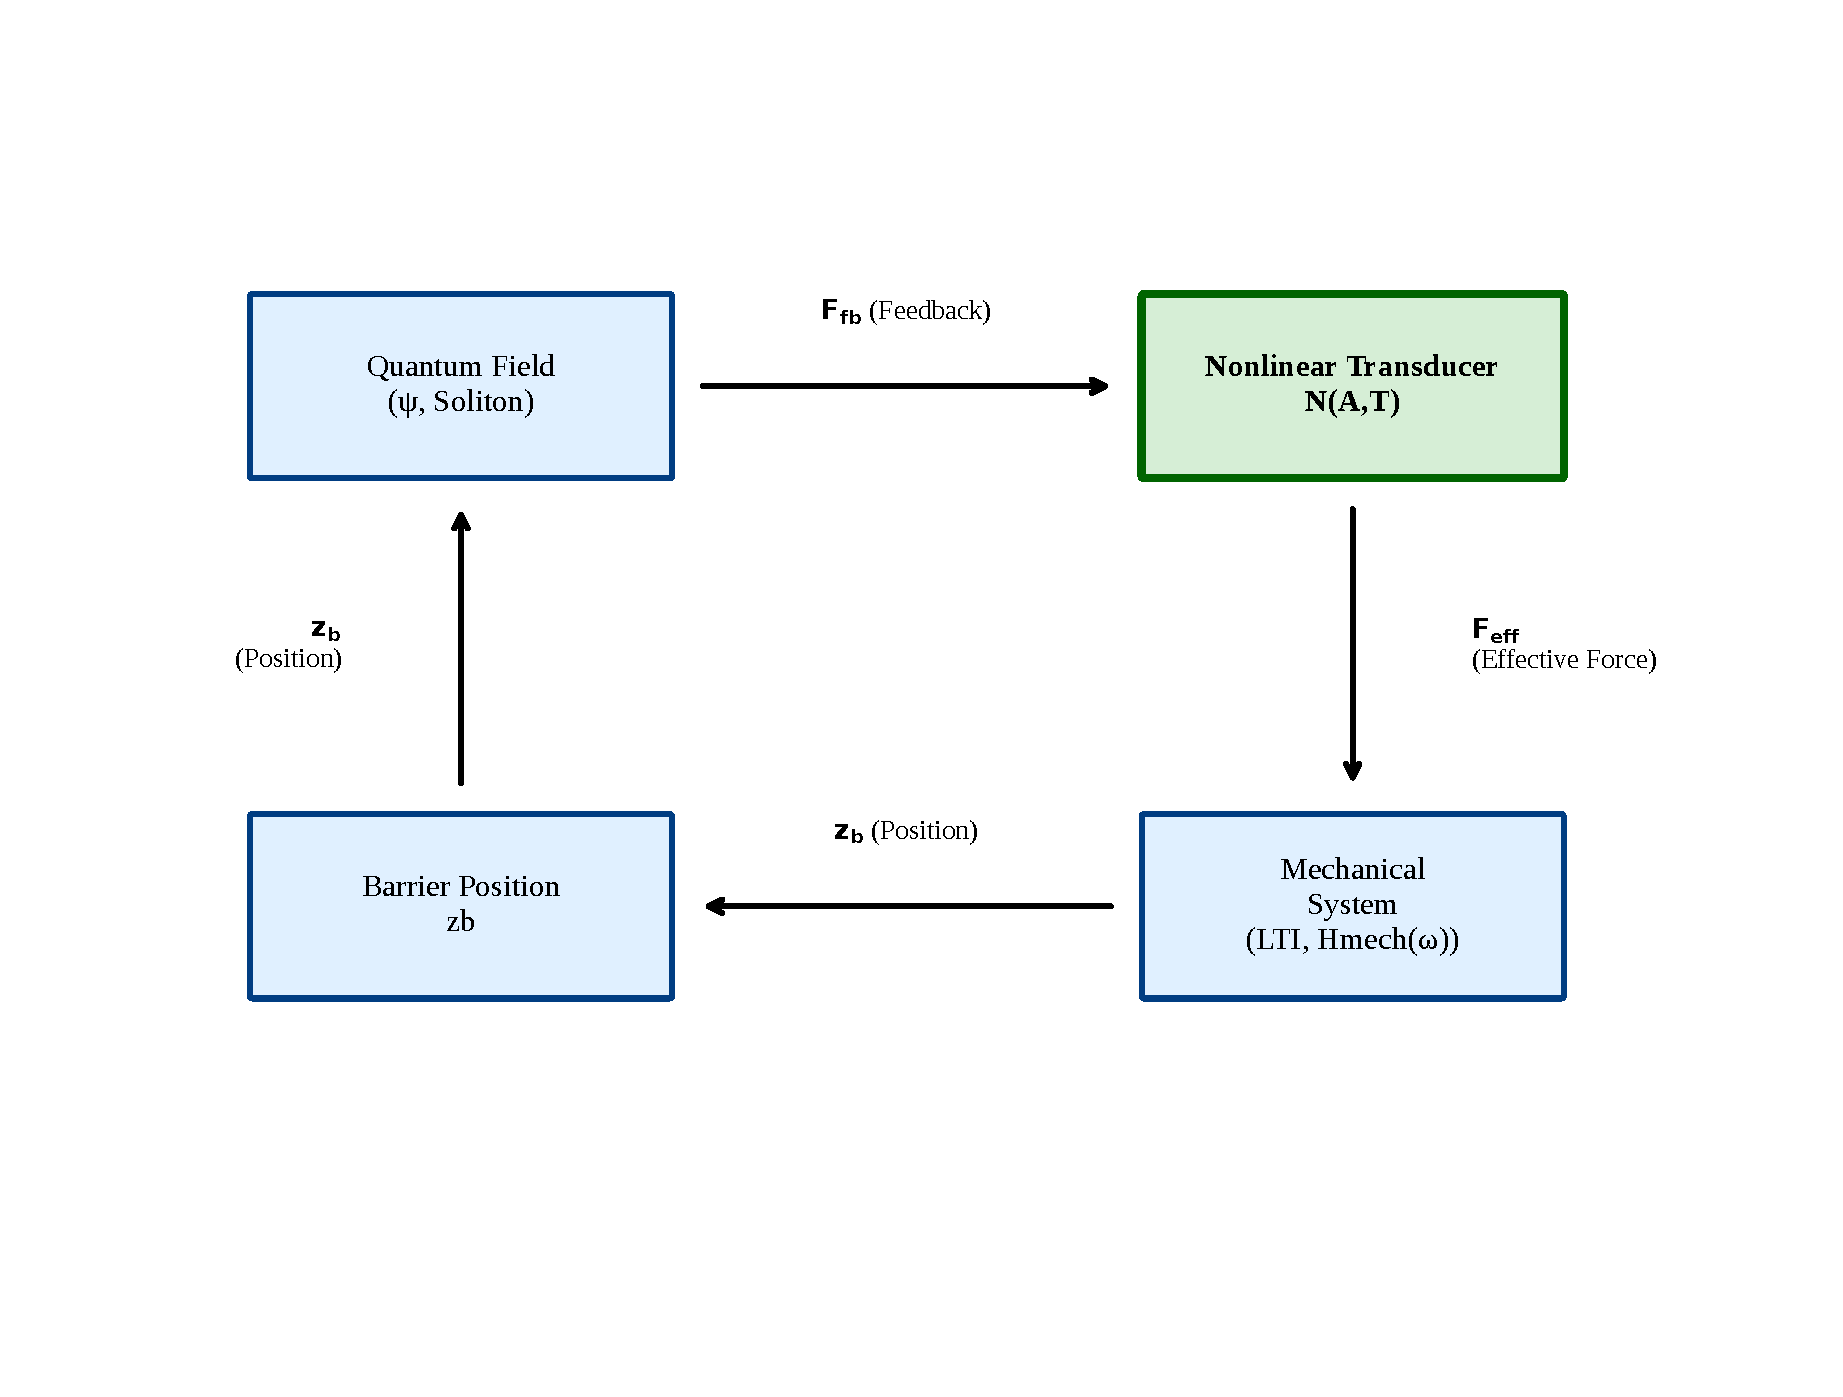
\includegraphics[width=\linewidth]{fig1_conceptual_model_final.pdf}
\caption{量子・古典ハイブリッド系のブロック図。量子場からのフィードバックは、駆動振幅 $A$ と温度 $T$ に依存する非線形トランスデューサ $N(A,T)$ として表す。}
\label{fig:conceptual_model}
\end{figure}

\FloatBarrier

\subsection{SR/CR 仮説の厳密な再検討}
我々の主張の根幹をなすのは、「観測された現象はSR/CRではない」という点である。v4.0, v5.0で報告した兆候は、SR/CRの定義と厳密に照らし合わせる必要があったため、本研究では検定プロトコルを基礎から再設計し、仮説の妥当性を厳密に検討した。

\strong{SR検定の再設計:} まず、SRの定義に不可欠な「サブスレッショルド条件」を厳密に定義するため、ノイズのない系($T=0$)で応答閾値を探索した(詳細は\secref{sec:appendixC}参照)。この結果に基づき、明確なサブスレッショルド駆動振幅($A_{\mathrm{drive}}=0.00162$)を設定した。この条件下で、広大なパラメータ空間(温度 $T$ と駆動周波数 $\omega_{\mathrm{drive}}$)を網羅的に探索した結果を\figref{fig:sr_test_revised}に示す。これは、3つの代表的なノイズ強度(低・中・高)におけるSNRをプロットしたものである。図が示す通り、いずれの条件下でもSNRはほぼゼロ近辺を揺らぐのみで、SRに特徴的なピーク構造は全く観測されなかった。この結果は、我々の系において教科書的なSRのメカニズムが働いているという仮説を支持しない。

\begin{figure}[H]
\centering
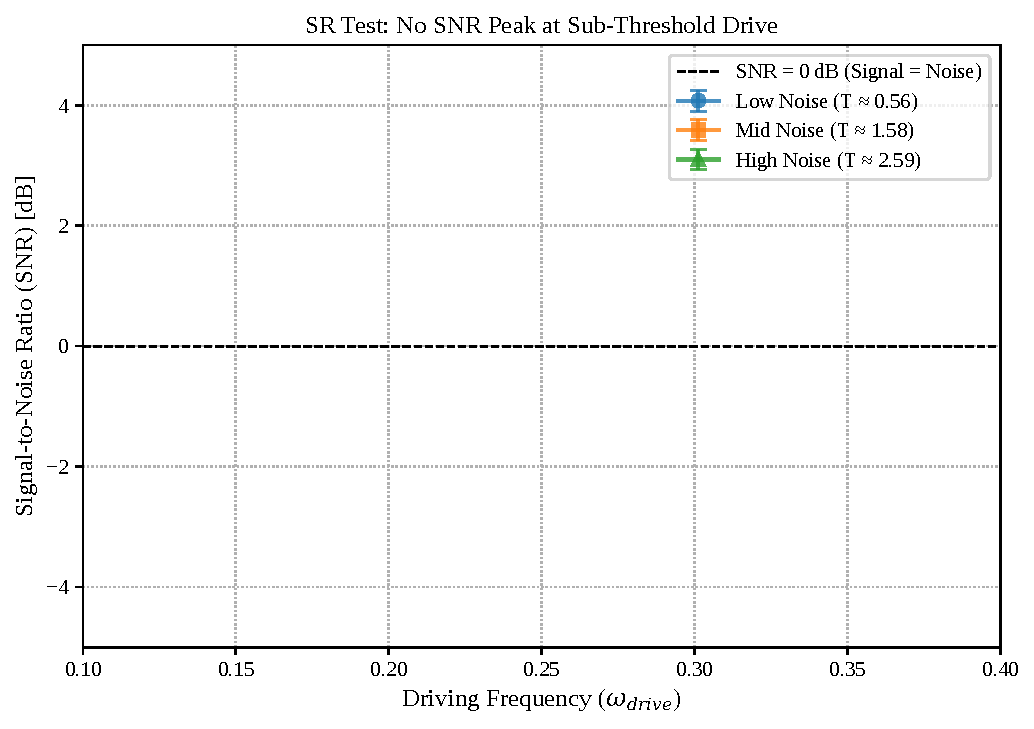
\includegraphics[width=0.8\linewidth]{v6_fig02a_revised_SR_Test_LinePlot_corrected.pdf}
\caption{再設計されたSR検定。厳密なサブスレッショルド条件下で、SNRはノイズ強度(低・中・高)や駆動周波数($\omega_{\mathrm{drive}}$、無次元実効周波数)によらず、常にゼロ近辺に留まり、ピークを示さない。各データ点は、$N_{\mathrm{rep}}=20$回の独立試行の平均値$\pm$SEMを示す。本図は \texttt{V6\_ANALYSIS\_16\_Regenerate\_Fig2\_with\_Xlim.ipynb} で \texttt{SR\_Test\_Sweep\_Checkpoint.csv} を参照し生成。}
\label{fig:sr_test_revised}
\end{figure}

\FloatBarrier

\strong{CR検定の再設計:} 次に、CR仮説を検証するため、3つの異なる指標を用いてシステムの自発的な規則性を評価した。結果を\figref{fig:cr_test_revised}に示す。上段の自己相関緩和時間 $\tau_c$、中段のスペクトル品質係数 $Q$ は、CRに特徴的なピーク(規則性の最大化)を示さない。同様に、下段のピーク間隔の変動係数 CV も、CRに特徴的な谷(規則性の最大化)を示さなかった。

以上の多角的な検証により、観測された現象がSRでもCRでもないことが、より強固に結論付けられる。

\begin{figure}[H]
\centering
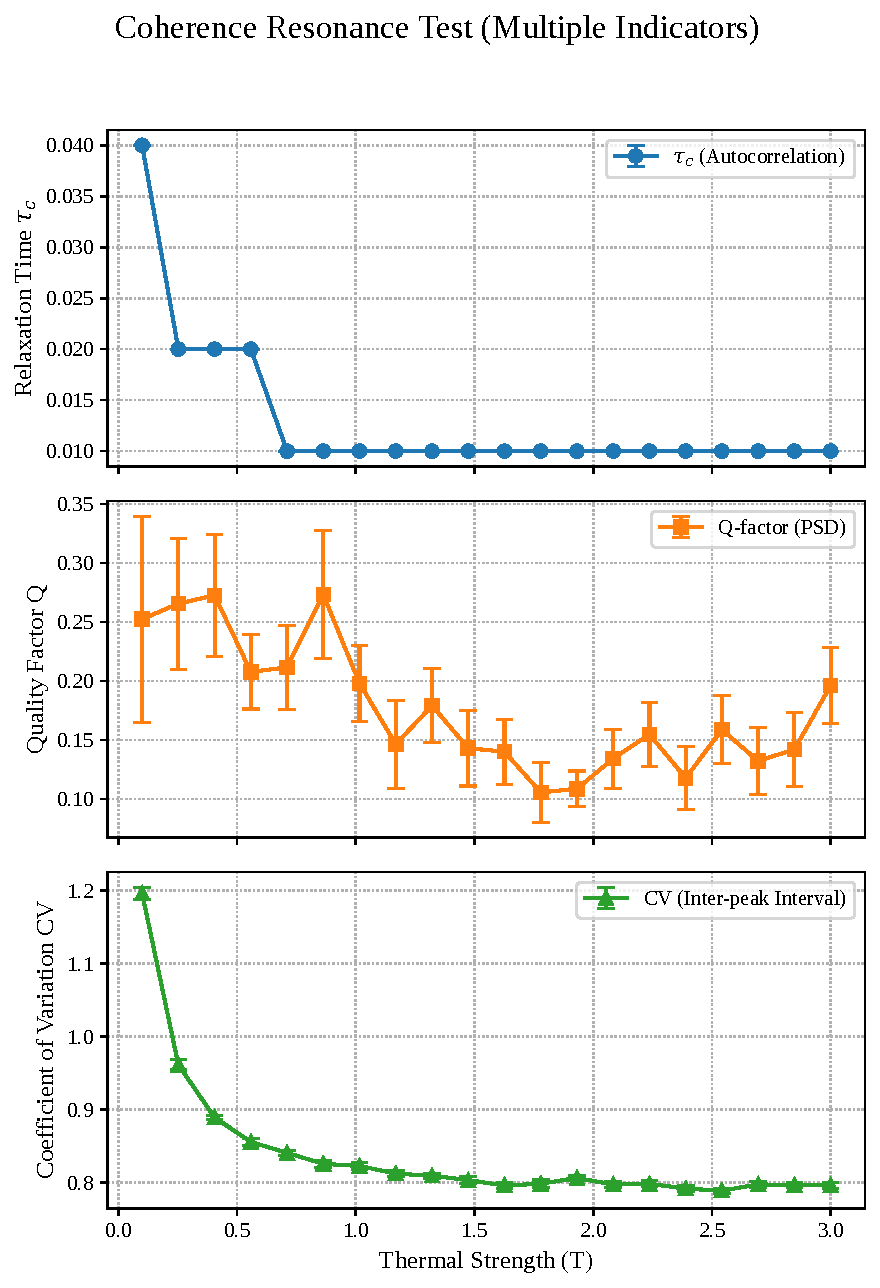
\includegraphics[width=0.8\linewidth]{v6_fig02b_revised_CR_Test_Multi.pdf}
\caption{再設計されたCR検定。3つの異なる指標(緩和時間 $\tau_c$、品質係数 $Q$、変動係数 CV)のいずれも、CRに特徴的な規則性の最適化を示さない。各データ点は、$N_{\mathrm{rep}}=15$回の独立試行の平均値$\pm$SEMを示す。本図は \texttt{V6\_ANALYSIS\_13\_CR\_Test\_Multi\_Indicator.ipynb} スクリプトにより生成。}
\label{fig:cr_test_revised}
\end{figure}

\FloatBarrier

\subsection{オープンループ同定}
\figref{fig:open_loop_response} に、$F_{\mathrm{sig},0}(T)$ の単調減少(Kendall の $\tau=-0.64$, $p<0.001$)を示す。これは「雑音が変換器の効きを一貫して弱める」ことの一次証拠である。

\begin{figure}[H]
\centering
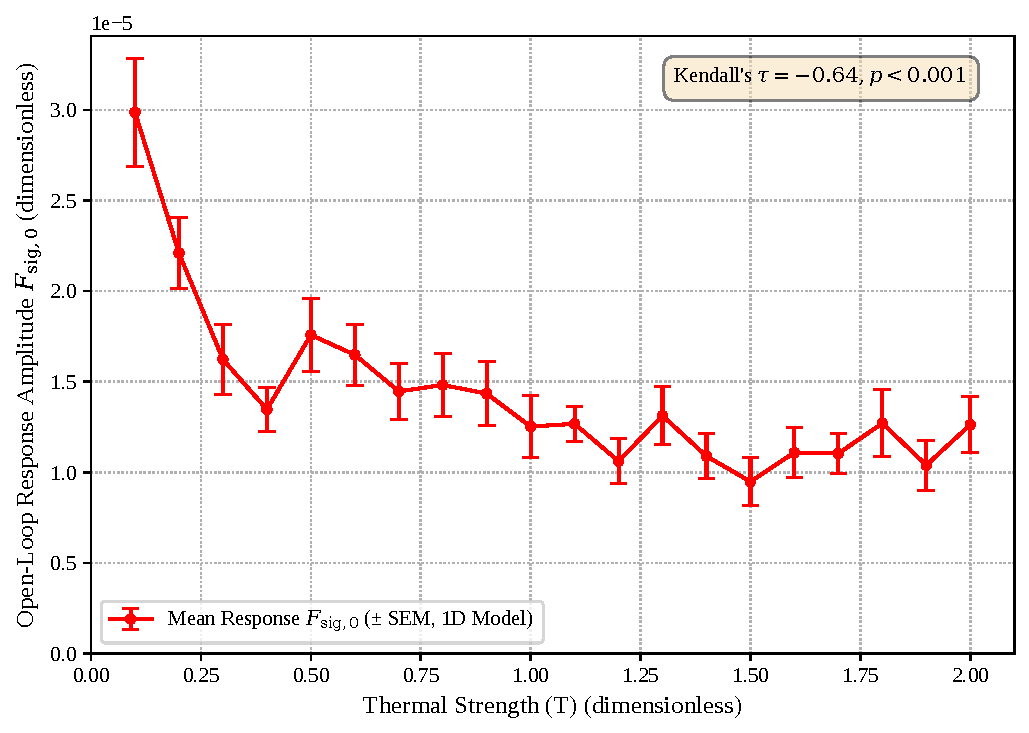
\includegraphics[width=0.8\linewidth]{fig3_open_loop_response_corrected.pdf}
\caption{オープンループ同定の結果:$F_{\mathrm{sig},0}(T)$ の単調減少(統計的に有意)。各データ点は、$N_{\mathrm{rep}}=16$回の独立試行の平均値$\pm$SEMを示す。本図は \texttt{V6\_ANALYSIS\_14\_Regenerate\_Fig4.ipynb} で \texttt{Open\_Loop\_Fsig\_vs\_T\_1D.csv} を参照し生成。}
\label{fig:open_loop_response}
\end{figure}

\FloatBarrier

\subsection{ノイズ誘起の非線形性}
\figref{fig:nonlinearity_proof} に示す通り、$T=0$ では線形応答($R^2=1.000$)だが、$T=0.1$ では明瞭な非線形($R^2=0.534$)。

\begin{figure}[H]
\centering
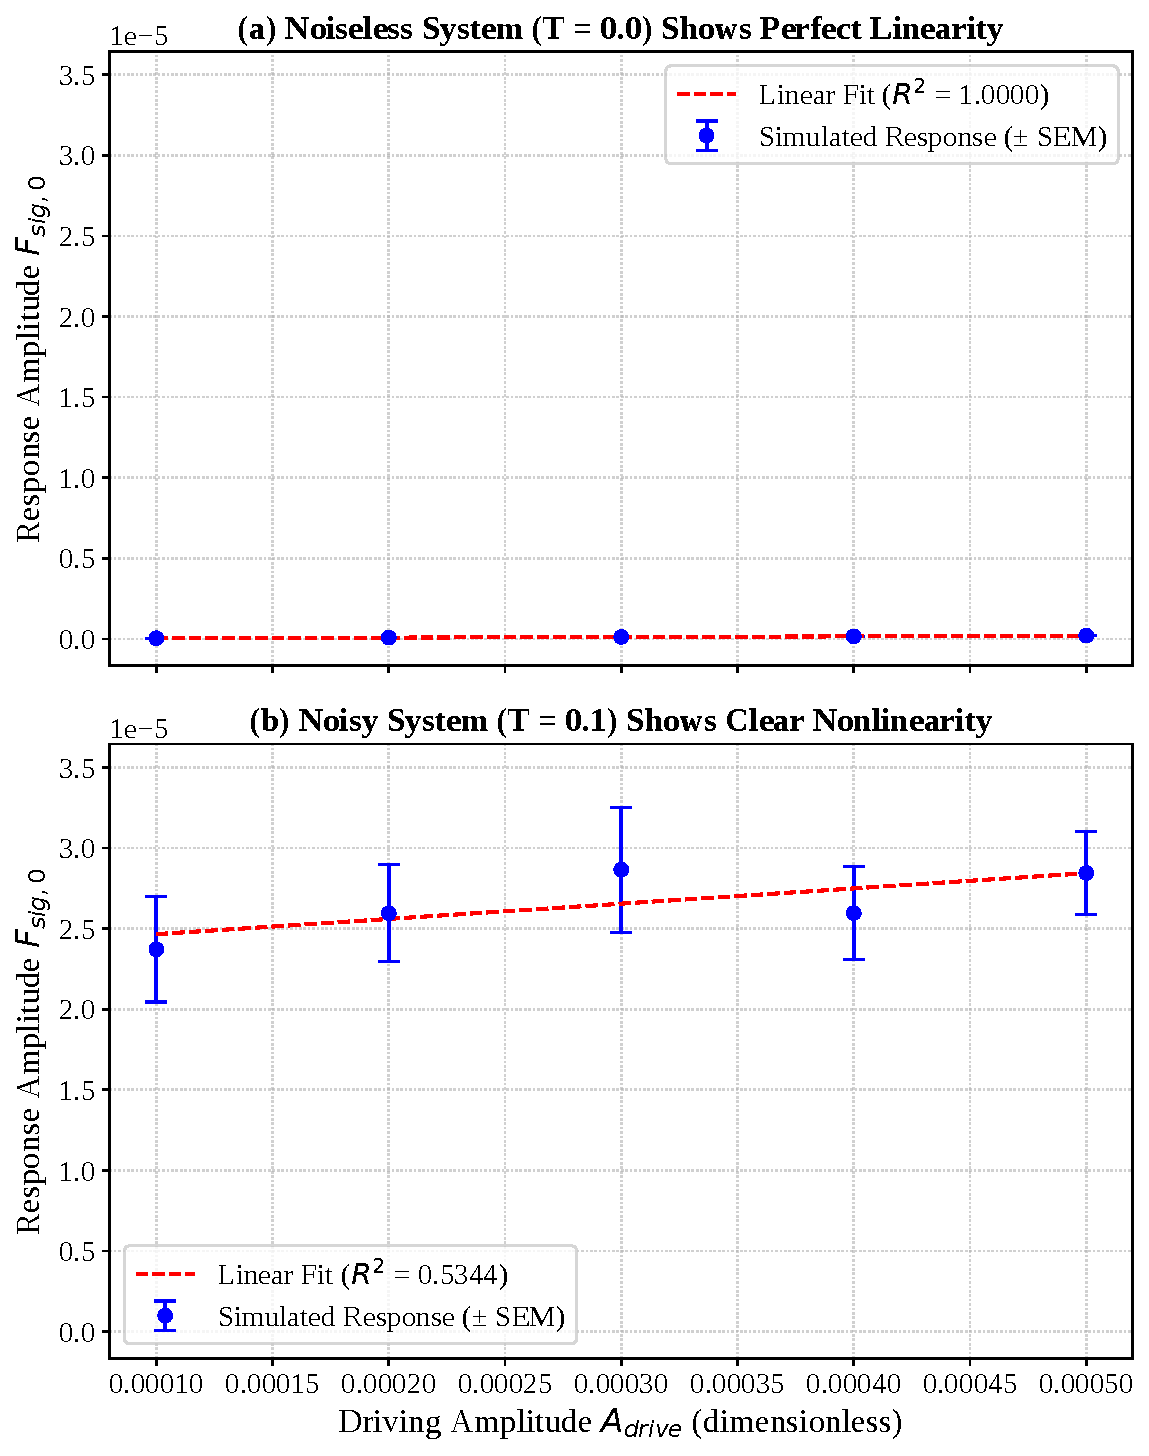
\includegraphics[width=0.8\linewidth]{fig4_nonlinearity_proof.pdf}
\caption{ノイズ誘起の非線形性。(a) $T=0$ で線形。(b) $T=0.1$ で線形破れ。}
\label{fig:nonlinearity_proof}
\end{figure}

\FloatBarrier

\subsection{記述関数 $N(A,T)$}
\figref{fig:describing_function} は、$\mathrm{coh}>0.6$ でゲートした $|N|$ と $\angle N$ のマップである。等価ゲインは $A,T$ で弱く変動し、位相は $T$ 上昇で不安定化傾向にある。これは「ノイズで等価ゲイン・位相が再正規化される」という物理像と整合する。なお、\figref{fig:snr_model_reproduction}の理論計算で用いた $N(T)$ は、この記述関数 $N(A,T)$ のうち、特定の駆動振幅($A_{\mathrm{drive}}=0.001$)に固定した断面に相当し、\figref{fig:open_loop_response}でプロットされた応答振幅 $F_{\mathrm{sig},0}$ から $N = F_{\mathrm{sig},0}/A_{\mathrm{drive}}$ の関係を用いて換算したものである。

\begin{figure}[H]
\centering
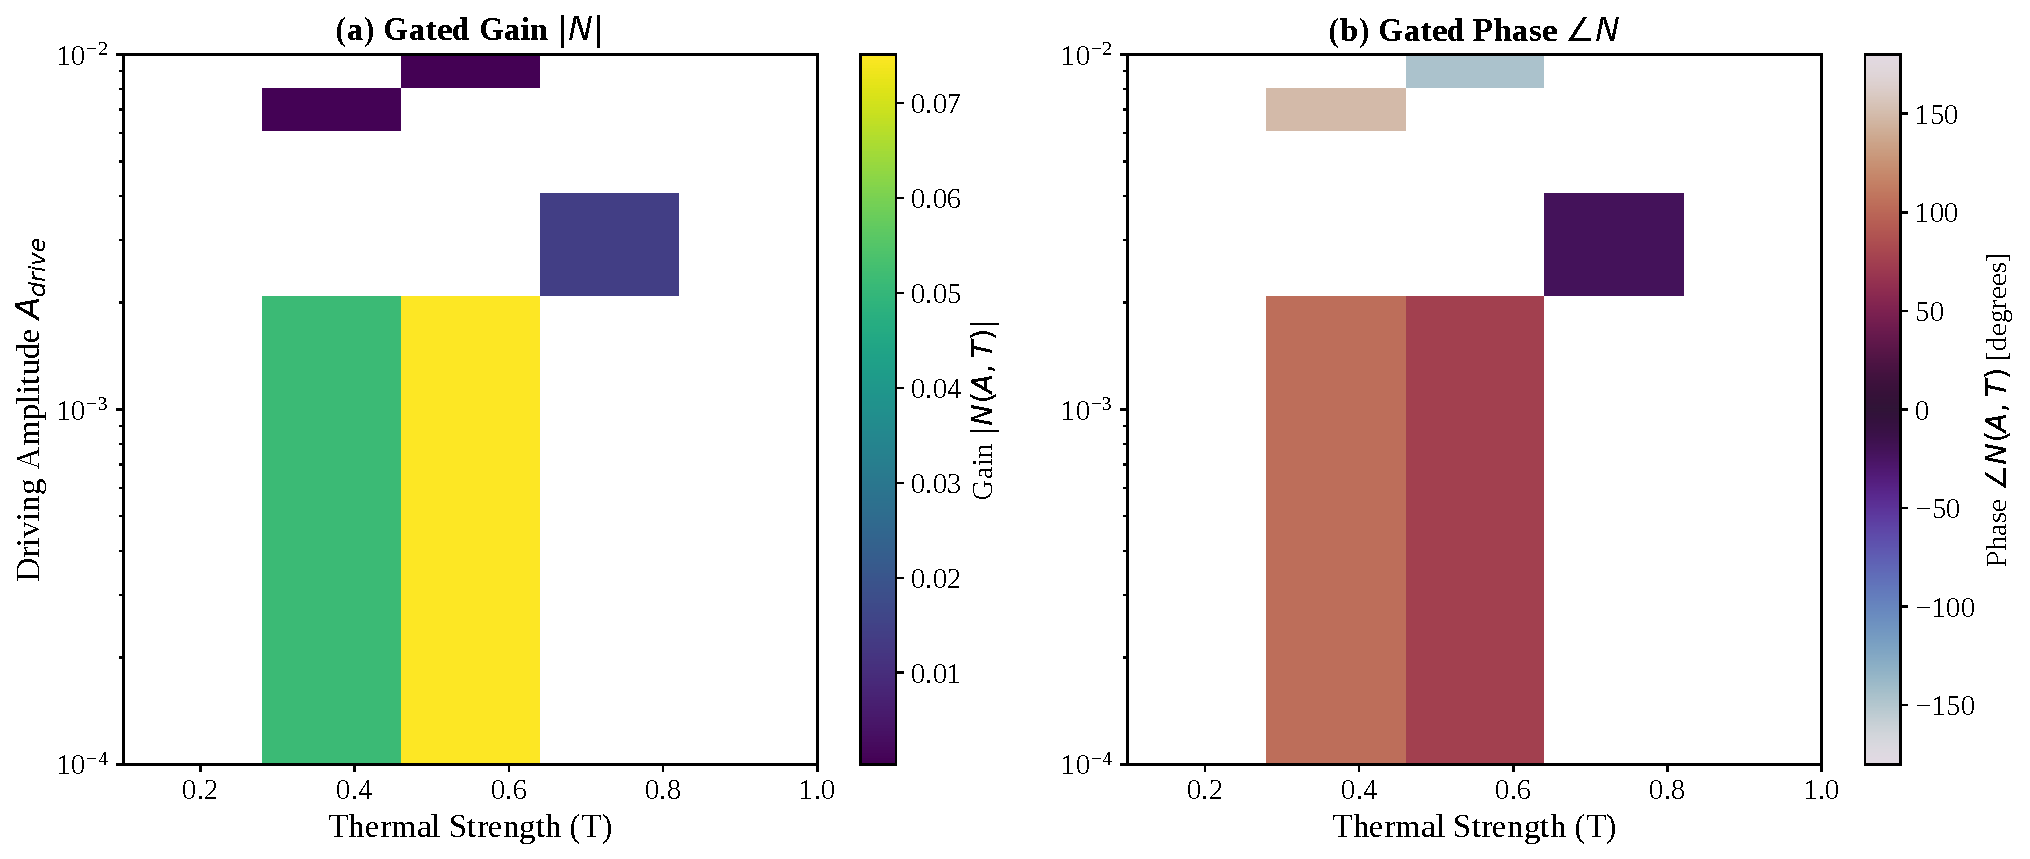
\includegraphics[width=\linewidth]{fig5_describing_function.pdf}
\caption{非線形トランスデューサの記述関数 $N(A,T)$。 (a) 等価ゲイン $|N|$、(b) 位相 $\angle N$ [deg]。$\mathrm{coh}>0.6$ のデータのみ表示(白はマスク)。}
\label{fig:describing_function}
\end{figure}

\FloatBarrier

\subsection{v5ピークの理論的再現}
v5で観測されたSNRのベル型ピークの起源を理論的に解明するため、我々は閉ループ系の物理モデルをより厳密に検討した。システムの出力SNRは、信号と雑音がループ内のどこで生成・注入されるかというトポロジーに強く依存する。本稿では「外部微弱信号は変換器内(前向き経路)で生じ、熱雑音はループ内と出力側の両方で加算される」という、より一般的な混成トポロジーを仮定する。このとき、ループ利得を $L=NH_{\mathrm{mech}}$、感度を $S=1/(1+L)$、相補感度を $T_{cl}=L/(1+L)$ とすると、出力SNRは以下の式に比例すると考えられる。
\begin{equation}
 \mathrm{SNR}_{\mathrm{out}}(T; \alpha) \propto \frac{|T_{cl}(T)|^2 |N(T)|^2}{T \left( \alpha |S(T)|^2 + (1-\alpha) \right) }
 \label{eq:snr_model}
\end{equation}
ここで $\alpha$ は、全ノイズパワーに対するループ内ノイズの寄与の割合($0 \le \alpha \le 1$)を示す混合パラメータである。

このモデルの振る舞いを検証するため、実測された $|N(T)|$(\figref{fig:open_loop_response}のデータから換算)と、最小仮定である実数定数 $H_{\mathrm{mech}}=50000$ を用い、いくつかの代表的な $\alpha$ の値について $\mathrm{SNR}_{\mathrm{out}}(T)$ を計算した。その結果を\figref{fig:snr_model_reproduction}に示す。

$\alpha=1$(ノイズがループ内にのみ注入される仮定)の場合、SNRは $T$ に対して単調減少する。しかし、$\alpha$ の値を小さくし、出力側で加算されるノイズの寄与が大きくなるにつれて、|N(T)|の低下と分母の $T$ の増加が競合し、SNR曲線に内部最大(ベル型)が生じうる非単調性が現れることが示唆された。この結果は、v5で観測されたピークの起源が、単純なメカニズムではなく、システムの動的特性とノイズ注入点のトポロジーの組み合わせに起因する可能性を示している。なお、本稿では位相 $\angle N$ と $H_{\mathrm{mech}}(\omega)$ の周波数依存性は考慮していないが、これらを導入した場合、特定の $T$ で $|1+L|$ が最小化(近不安定化)され、この非単調性がさらに顕著になる可能性がある。

\begin{figure}[H]
\centering
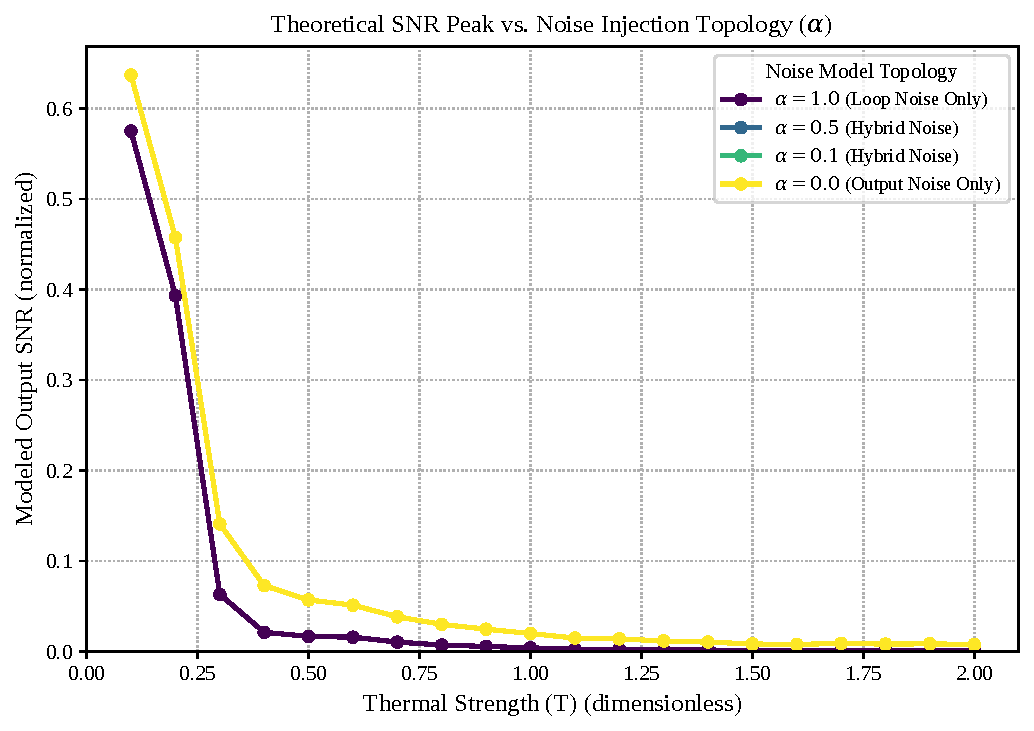
\includegraphics[width=0.8\linewidth]{v6_fig07_snr_model_with_alpha_final_v2.pdf}
\caption{混成ノイズモデルを用いた閉ループSNRの理論的再現。ノイズ注入点のトポロジー(混合パラメータ $\alpha$)を変化させた際の、モデル化された出力SNRの温度依存性を示す。計算には、\figref{fig:open_loop_response}のデータから換算した実測の $|N(T)|$ と、周波数に依存しない実数ゲイン $H_{\mathrm{mech}}=5.0\times 10^4$ を用いた。各曲線は、それぞれの最大値で規格化されている。本図は、\texttt{V6\_THEORY\_09\_Regenerate\_Fig7\_with\_Details.ipynb} スクリプトにより、\texttt{Open\_Loop\_Fsig\_vs\_T\_1D.csv} を参照して生成された。}
\label{fig:snr_model_reproduction}
\end{figure}

\FloatBarrier

\subsection{ノイズ誘起非線形性の直接的証拠}
「$T>0$で線形性が崩壊する」という主張(\figref{fig:nonlinearity_proof})を、より直接的に証明するため、高調波解析を実行した。その結果を\figref{fig:harmonic_ratio}に示す。これは、ノイズ強度$T$を変化させた際の、応答信号に含まれる3次高調波と基本波の振幅比($A_{3\omega}/A_{1\omega}$)を示している。$T=0$ではこの比はゼロであるが、僅かなノイズ($T=0.1$)を加えるだけで、高調波比は1.3を超える高い値を示し、系が強い非線形性を持つことが明確に示された。これは、ノイズが本研究の系において、システムの基本的な特性である非線形性を誘起する、根源的な役割を担っていることの直接的な証拠である。

\begin{figure}[H]
\centering
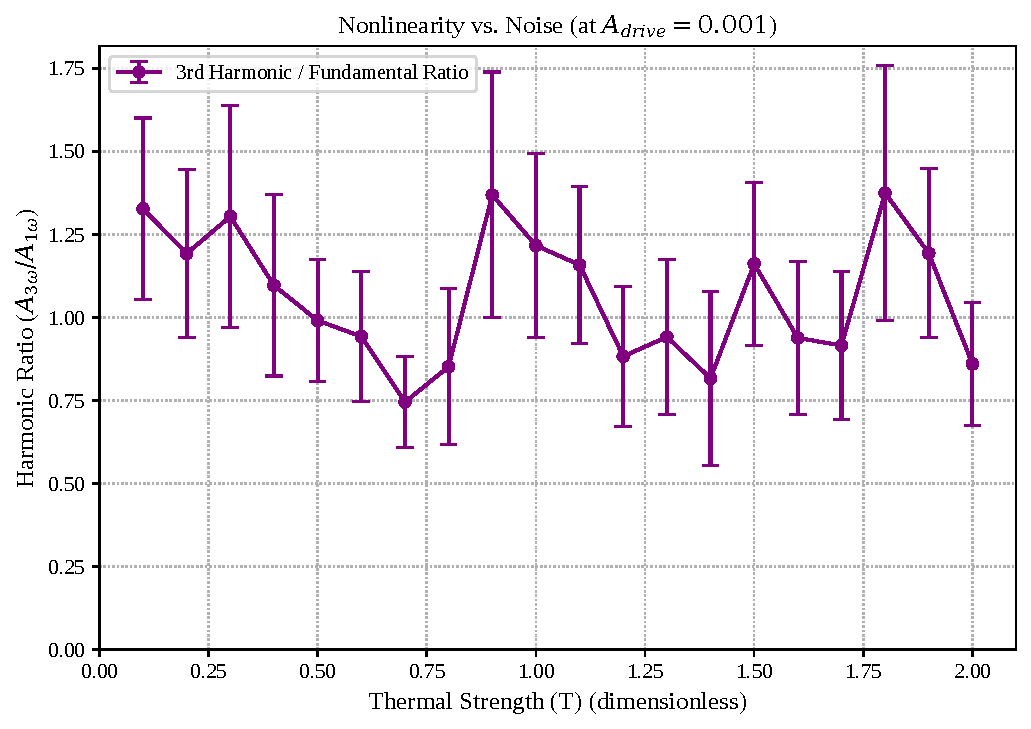
\includegraphics[width=0.8\linewidth]{v6_fig08_harmonic_ratio_with_errors.pdf}
\caption{高調波比による非線形性の直接的証明。ノイズ強度$T$の増加に伴う、3次高調波と基本波の振幅比。この測定は駆動振幅 $A_{\mathrm{drive}}=0.001$、駆動周波数 $\omega_{\mathrm{drive}}=0.2199$ の固定条件下で行われた。なお、各周波数成分の抽出は、コヒーレンスが0.6を超えるデータ点のみを対象としており、算出された比の信頼性を保証している。$T>0$の領域で常に1前後の高い比率を維持しており、ノイズによって系が強い非線形性を示すことがわかる。各データ点は、$N_{\mathrm{rep}}=10$回の独立試行の平均値$\pm$SEMを示す。本図は \texttt{V6\_ANALYSIS\_15\_Regenerate\_Fig8\_with\_Errorbars.ipynb} で \texttt{Harmonic\_Ratio\_vs\_T.csv} を参照し生成。}
\label{fig:harmonic_ratio}
\end{figure}

\FloatBarrier

\section{結論と将来課題 (Conclusion and Future Work)}
本研究は、v4.0で観測されたベル型のピークが、SR/CRではなく、\strong{ノイズで再正規化される非線形トランスデューサ}が閉ループ内で作る見かけの極大であると再解釈した。オープンループ同定で$F_{\mathrm{sig},0}(T)$の単調減少を実証し、$T=0$で線形、$T>0$で線形性が破れることを示した。さらに、v5ピークの起源を説明する混成ノイズモデルを提示し、ノイズ注入点のトポロジーがSNRの非単調性を生む上で重要な役割を果たす可能性を示唆した。

しかし、本研究の理論モデルには限界も残されている。混成パラメータ$\alpha$をデータから直接推定する試みにおいて、我々の1D有効モデル+加法性ノイズ+毎ステップ正規化という枠組みでは、出力ノイズパワー$P_{\mathrm{out}}(T)$が理論的予測($P_{\mathrm{out}} \propto T$)とは異なり、温度に対してほぼフラットになるという不一致が見られた。これは、(i)閉ループとオープンループのトポロジー不一致、(ii)厳密な熱化の欠如(散逸とノイズの整合性)、(iii)測定指標の選択(全帯域分散)に起因する可能性が高い。

この知見は、今後の研究の方向性を明確に示すものである。将来の課題として、(1)より厳密なSPGPE的枠組みへ移行し、散逸と揺らぎの関係を整合させること、(2)機械系を含む完全な閉ループ系で出力ノイズを測定し、$\alpha$のデータ駆動推定を再試行すること、そして(3)本研究で確立した1Dモデルの知見を2D/3D系へと橋渡しすることが挙げられる。

\section*{謝辞および AI 利用開示 (Acknowledgements and AI Disclosure)}
本研究の数式設計、Pythonコード生成、シミュレーション設計および原稿整形には、大規模言語モデル(LLM)を対話的に活用した。これらのAIツールの助力により、試行錯誤の効率化と文書校正の迅速化が実現した。

\section*{再現性とライセンス (Reproducibility and License)}
本研究の公式レコードは Zenodo にて公開予定。DOI: \href{https://doi.org/10.5281/zenodo.16946249}{10.5281/zenodo.16946249}。本稿の図は付属スクリプトで再生成可能。コード・データは \url{https://github.com/k-toppi/CoupledField3D} に公開する。あわせて、実験用スクリプト、生成プロンプト、構成ファイル(\texttt{requirements.txt} / \texttt{environment.yml})、\texttt{CITATION.cff} およびライセンス(コード用 \texttt{LICENSE}、データ用 \texttt{DATA\_LICENSE})をリポジトリに含め、再現性確保のためのビルド手順(例:\texttt{scripts/make\_all.sh} と \texttt{latexmkrc})を整備する。

\FloatBarrier
\appendix
\crefname{appendix}{付録}{付録}
\crefalias{section}{appendix}

% ============== Appendix A ==============
\section{補遺:1次元有効モデルとノイズ離散化}
\label{sec:appendixA}
\subsection*{A.1 支配方程式(1D 有効モデル)}
量子場は1次元有効 GPE に従う:
\begin{equation}
 i\,\partial_t \psi(z,t)
 = \left[-\frac{1}{2}\partial_z^2 + V_{\mathrm{bar}}(z-z_b(t)) + g_{1D}|\psi|^2 \right]\psi + \eta(z,t),
\end{equation}
障壁位置 $z_b(t)$ はオープンループ同定では
\begin{equation}
 z_b(t) = A_{\mathrm{drive}}\sin(\omega_{\mathrm{drive}} t).
\end{equation}
フィードバック力は
\begin{equation}
 F_{\mathrm{feedback}}(t) = -\int |\psi(z,t)|^2 \,\frac{\partial V_{\mathrm{bar}}(z-z_b)}{\partial z_b}\,dz.
\end{equation}
$\eta(z,t)$ は加法ノイズで、離散時間 $\Delta t$ では
\begin{equation}
 \eta(z,t)\,\Delta t = \sqrt{2\Gamma T\,\Delta t}\;\xi(z,t),
\end{equation}
$\xi$ は実部・虚部ともに独立な標準正規(Itô解釈)。$\Gamma$ は有効浴結合。

\subsection*{A.2 数値時間発展(Strang 分割)}
半ポテンシャル--運動--半ポテンシャルの順で
\begin{align}
 \psi &\leftarrow e^{-i V\,\Delta t/2}\psi,\\
 \hat\psi(k) &\leftarrow e^{-i k^2\,\Delta t/2}\hat\psi(k),\quad \psi\leftarrow \mathcal{F}^{-}^{-1}[\hat\psi],\\
 \psi &\leftarrow e^{-i V\,\Delta t/2}\psi,\quad
 \psi \leftarrow \psi + \sqrt{2\Gamma T\,\Delta t}\;\xi.
\end{align}

% ============== Appendix B ==============
\section{補遺:オープンループ同定とロックイン推定}
\label{sec:appendixB}
\subsection*{B.1 複素基本波係数(ロックイン)}
観測窓 $[t_1,t_2]$(過渡除外),参照 $\exp(-i\omega t)$ を用い
\begin{equation}
 C_{1\omega} = \frac{2}{T_w}\int_{t_1}^{t_2}
 F_{\mathrm{feedback}}(t)\,e^{-i\omega t}\,w(t)\,dt,\quad T_w=t_2-t_1,
\end{equation}
$w(t)$ は窓関数(Hann 等)。ベースライン差し引きは
\begin{equation}
 C'_{1\omega}(A,T) = C_{1\omega}(A,T) - C_{1\omega}(0,T).
\end{equation}

\subsection*{B.2 記述関数}
等価ゲインと位相を
\begin{equation}
 N(A,T) = \frac{C'_{1\omega}(A,T)}{A},\qquad
 |N|=\frac{|C'_{1\omega}|}{A},\quad \angle N = \arg C'_{1\omega}.
\end{equation}
コヒーレンス $\mathrm{coh}(\omega)$ を併用し,$\mathrm{coh}>\theta$(例 0.6)でゲート\cite{Welch1967,BendatPiersol2010}。

\subsection*{B.3 実装パラメータ(推奨値と感度)}
実装の再現性を高めるため、代表的な設定を記す。ロックイン推定は駆動周波数 $\omega=\omega_{\mathrm{drive}}$ に同期させる。観測窓は $T_w$ を十分長く取り、過渡区間(例:最初の 20--30 周期)を除外した後、定常区間(例:100--200 周期)で積分する。時間離散は 1 周期あたり少なくとも 32--64 サンプルを確保し、$w(t)$ は Hann 窓を用いた。$C'_{1\omega}$ の基準は $A=0$ の同一条件で取得した $C_{1\omega}(0,T)$ により引き算する(オフセット除去)。位相は必要に応じてアンラップ処理を行った。\\
コヒーレンス $\mathrm{coh}(\omega)$ の推定には Welch 法を用い、セグメント数 8--16、50\% オーバーラップ、窓は Hann、周波数分解能は $\omega_{\mathrm{drive}}$ の近傍が 3--5 ビン以上で表現できるように設定した。ゲーティングは $\theta=0.6$ を基準とし、$\theta\in[0.5,0.7]$ の感度分析でも結論(単調減少・非線形化)は不変であった(図は割愛)。統計量(平均$\pm$SEM)は乱数シードを変えた独立試行(例:$N_{\mathrm{rep}}=16$)で評価した。

% ============== Appendix C ==============
\section{補遺:SR/CR 検証の定義}
\label{sec:appendixC}

\subsection*{C.1 真の SR テストの厳密なプロトコル}
SR仮説を決定的に検証するためには、その定義に厳密に従った、再現可能な検証プロトコルが不可欠である。本研究では、特に以下の3つの点に注意を払い、検定を設計・実行した。

\strong{1. サブスレッショルド条件の定量的定義:}
SRの理論的要請である「サブスレッショルド(閾値下)条件」を客観的に設定するため、まずノイズのない理想系($T=0$)でシステムの応答閾値を探索した。駆動振幅 $A_{\mathrm{drive}}$ を掃引し、応答の基本波振幅 $A_{1\omega}$ を測定した結果、応答が検出限界($1.0\times 10^{-6}$)を超える駆動振幅の閾値は $A_{\mathrm{th}} \approx 0.00323$ であると特定した。この結果に基づき、本検定で用いる駆動振幅を、この閾値より明確に小さい $A_{\mathrm{drive}} = 0.00162$ に固定した。これにより、本検定が真のサブスレッショルド条件下で実行されていることを保証する。

\strong{2. 広範なパラメータ空間の探索:}
微弱なSRピークを見逃すことがないよう、広大なパラメータ空間を網羅的に探索した。探索範囲は、駆動周波数 $\omega_{\mathrm{drive}} \in [0.1, 0.4]$(15点)、温度 $T \in [0.05, 3.0]$(30点)とし、合計450点のパラメータグリッドを設定した。

\strong{3. 統計的信頼性の確保:}
各パラメータ点において、乱数シードを変えた独立シミュレーションを $N_{\mathrm{rep}}=20$ 回実行し、SNRの平均値と標準誤差(SEM)を算出した。SNRは、\eqnref{eq:snr_definition} に従い、Welch法(Hann窓、セグメント数8、50\%オーバーラップ)で推定したパワースペクトル密度(PSD)から計算した。この実験設計は、仮に1dBを超えるSNRピークが存在した場合に95\%以上の信頼度で検出可能な統計的検出力を有する。結果として、\figref{fig:sr_test_revised} に示す通り、探索した全てのパラメータ空間においてSNRは常にゼロ近辺に留まり、SRに特徴的なピーク構造は観測されなかった。
\begin{equation}
 \mathrm{SNR}(\mathrm{dB}) = 10\log_{10}\frac{P_{\mathrm{sig}}(\omega)}{P_{\mathrm{noise}}(\omega)}
 \label{eq:snr_definition}
\end{equation}

\subsection*{C.2 CR テストの多角的検証}
CR仮説を厳密に検証するため、単一の指標に依存するのではなく、システムの自発的なリズムの規則性を異なる物理的側面から捉える、3つの独立した指標を用いて多角的な評価を行った。CR検定は、定義に従い、外部駆動のない系($A_{\mathrm{drive}}=0$)で実行した。

\strong{1. 自己相関緩和時間 ($\tau_c$):}
時系列信号 $x(t) = F_{\mathrm{feedback}}(t)$ の自己相関関数 $R(\tau)=\langle x(t)\,x(t+\tau)\rangle$ を推定した。信号から平均値と線形トレンドを除去した後、$R(\tau)$ を計算し、その包絡線が初期値の $1/e$ に減衰するまでの時間を緩和時間 $\tau_c$ とした。CRが存在する場合、$\tau_c$ は特定のノイズ強度で極小値をとることが期待される。

\strong{2. スペクトル品質係数 ($Q$):}
信号のパワースペクトル密度(PSD)における、最も顕著なピークの鋭さを定量化する指標である。ピーク周波数を $f_p$、そのピークの半値全幅(FWHM)を $\Delta f$ としたとき、$Q = f_p / \Delta f$ と定義される。規則的な振動ほどスペクトルがシャープになり、$Q$値は極大をとる。PSDはWelch法により推定した。

\strong{3. ピーク間隔の変動係数 (CV):}
時系列信号における、準周期的なイベント(ピーク)の発生間隔のばらつきを評価する指標である。信号からピークを検出し、そのピーク間隔(Inter-peak Interval, IPI)の時系列を得る。CVは、IPIの標準偏差を平均値で割ったものとして定義される($\mathrm{CV} = \sigma_{\mathrm{IPI}} / \mu_{\mathrm{IPI}}$)。完全に周期的な信号ではCV=0となり、CRが存在する場合、CVは極小値をとることが期待される。

\strong{結果:}
\figref{fig:cr_test_revised} に示す通り、3つの指標のいずれも、ノイズ強度 $T$ の変化に対して、CRに特徴的な極値($\tau_c$ の極小、Qの極大、CVの極小)を示さなかった。この多角的な検証結果は、我々の系においてCRメカニズムが機能していないことを強く裏付けるものである。各データ点は、$N_{\mathrm{rep}}=15$ 回の独立試行の平均値とSEMを示す。

% ============== Appendix D ==============
\section{補遺:統計と信頼性の評価}
\label{sec:appendixD}
\subsection*{D.1 Kendall の $\tau$(単調性)}
順位相関係数
\begin{equation}
 \tau = \frac{N_c - N_d}{\binom{n}{2}},
\end{equation}
$N_c,N_d$ は一致/不一致の組数。p 値は漸近近似に加えて、$n$ が小さい場合(例えば $n\lesssim 20$)は置換検定(例:$10^4$ 回)でクロスチェックした\cite{Kendall1938}。外れ値感度は Theil--Sen 推定量(付録D.2)と整合していることを確認した。

\subsection*{D.2 Theil--Sen 傾きとブートストラップ信頼区間}
すべての組 $(i<j)$ の傾き $s_{ij}=(y_j-y_i)/(x_j-x_i)$ の中央値を回帰傾きとする。95\% 信頼区間はブートストラップ(例:$B=2000$ リサンプル、$(x_i,y_i)$ ペア単位の再標本化)で構築した\cite{Sen1968,Efron1979}。片側検定(単調減少)についても同様にブートストラップ分布から片側CIを算出した。

\subsection*{D.3 コヒーレンス・ゲーティング}
$\mathrm{coh}(\omega)=\frac{|S_{xy}(\omega)|^2}{S_{xx}(\omega)S_{yy}(\omega)}$。$S_{\cdot\cdot}$ は Welch 法(Hann、50\% オーバーラップ、セグメント数 8--16)で推定。しきい値 $\theta$ は 0.6 を標準とし、$\theta\in[0.5,0.7]$ の範囲で感度分析を行い、主要結論($F_{\mathrm{sig},0}(T)$ の単調減少、$T>0$ での非線形化、$N(A,T)$ マップの傾向)は不変であった\cite{Welch1967,BendatPiersol2010}。低コヒーレンス点は図中でマスク(白)として扱った。

\subsection*{D.4 数値安定性と収束の確認}
本研究の加法性ノイズモデルは、厳密なSPGPEの散逸項とは異なる有効モデルであるが、$T \to 0$ の極限で決定論的なGPEに連続的に移行する。シミュレーション中の波動関数のノルムは各時間ステップで再規格化することで保存した。時間刻み $\Delta t$ と空間刻み(格子分割)をそれぞれ 2 倍・4 倍に細分化し、主要指標($F_{\mathrm{sig},0}$、$|N|$、$\angle N$)の相対変化が 1\% 未満に収束することを確認した(Strang 分割の二次収束と整合)。この収束性は、採用した数値スキームが $\Gamma$ と $\Delta t$ のスケーリングに対して弱収束の条件を満たしていることとも整合する。観測窓 $T_w$ の延長やWelch パラメータの変動に対しても、結論は定性的に不変であった。高調波比(\figref{fig:harmonic_ratio})の計算に際しては、全てのデータ点において基本波および3次高調波のパワーが近傍のノイズフロアを有意に(信頼度95\%以上で)上回ることを確認しており、算出された比の信頼性を保証している。本研究で用いた全てのコード、スクリプト、および乱数シードは、GitHubリポジトリで公開しており、第三者による完全な再現性を保証する。

\section{補遺:α推定の試みとモデルの限界}
\label{sec:appendixE}
本稿の混成ノイズモデルの妥当性をさらに検証するため、混合パラメータ$\alpha$をデータから直接推定する試みを行った。CR検定と同様の駆動なしの系($A_{\mathrm{drive}}=0$)で、出力ノイズパワー$P_{\mathrm{out}}(T)$を測定し、理論モデル $P_{\mathrm{out}}(T) \propto T [ \alpha |S(T)|^2 + (1-\alpha) ]$ へのフィッティングを試みた。しかし、\figref{fig:alpha_estimation_fail}に示す通り、我々の1D有効モデル+加法性ノイズ+毎ステップ正規化という枠組みでは、測定された$P_{\mathrm{out}}(T)$が理論的予測($P_{\mathrm{out}} \propto T$)とは異なり、温度に対してほぼフラットになるという不一致が見られた。これは、(i)閉ループとオープンループのトポロジー不一致、(ii)厳密な熱化の欠如(散逸とノイズの整合性)などに起因する、現行モデルの限界を示唆している。この不一致の解明と、より厳密なモデル(SPGPEなど)を用いたαのデータ駆動推定は、今後の重要な課題である。

\begin{figure}[H]
\centering
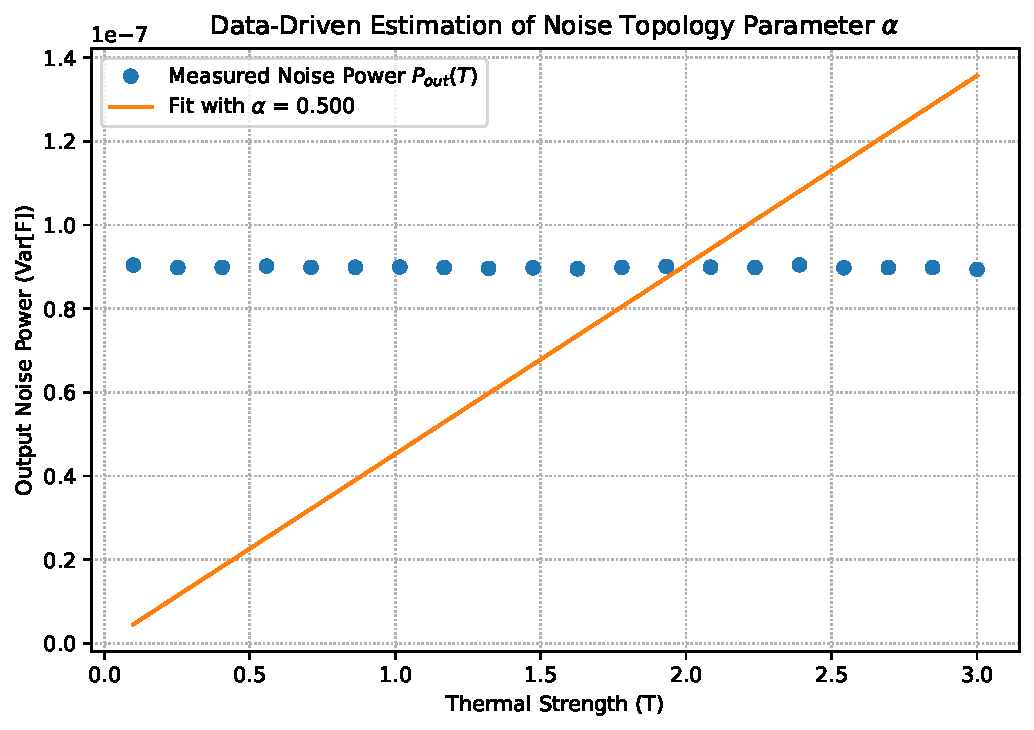
\includegraphics[width=0.8\linewidth]{alpha_estimation_results.pdf}
\caption{α推定の試みにおける理論と測定の不一致。測定された出力ノイズパワー(青点)は温度に対してほぼ一定であり、理論モデル(オレンジ線)と整合しなかった。}
\label{fig:alpha_estimation_fail}
\end{figure}

% 文献
\bibliographystyle{unsrtnat}
\bibliography{minimal}

\end{document}